\documentclass[11pt,letterpaper,twoside]{article}
\usepackage[english]{babel}
\usepackage{amssymb,amsmath}
\usepackage{fancyhdr}
\usepackage{graphicx}

 \oddsidemargin  0in \evensidemargin 0in
 \topmargin   -0.25in \headheight 0.25in \headsep 0.25in
 \textwidth   6.5in \textheight 8.75in \marginparsep 0pt \marginparwidth 0pt
 \parskip 1ex  \parindent 0ex \footskip 20pt

\newfont{\bssten}{cmssbx10}
\newfont{\bssnine}{cmssbx10 scaled 900}

%%%%%%%%%%%%%%%%%%%%%%%
\newcommand{\whatizit}{Lecture 1: Introduction and Case Study}
%%%%%%%%%%%%%%%%%%%%%%%


\pagestyle{fancy}  
\fancyhead{\bssnine STOR 155,  \whatizit}
\fancyhead[RE]{} \fancyhead[LO]{}
\fancyhead[LE]{\bssnine \thepage} \fancyhead[RO]{\bssnine \thepage}
\lfoot{} \cfoot{} \rfoot{}   


\newcommand{\var}{\mathrm{Var}}



\begin{document}



\thispagestyle{empty} \vspace*{-0.75in}

{\bssten STOR 155: Introduction to Data Models and Inference \hfill May 15, 2024 \\
Prof. Will Lassiter  \hfill Page 1 of \pageref{totalpag}}
\vspace{10pt}
\begin{center} {{\Large \bf \whatizit}} \end{center}

{\bf Course Overview}: What do we learn?

\begin{enumerate}

\item {\bf Identify a question or problem of interest} \vspace{50pt}

\item {\bf Collect relevant data} \vspace{50pt}

\item {\bf Analyze the data} \vspace{50pt}

\item {\bf Form a conclusion} \vspace{50pt}

\end{enumerate}

{\bf Case Study}: Do stents reduce the risk of stroke in at-risk patients?

\begin{center}
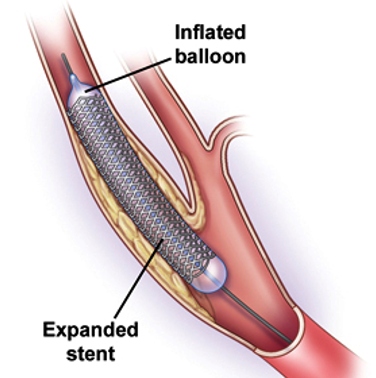
\includegraphics[scale=1]{stent.png}
\end{center}

Stents have been suggested as a tool for reducing the risk of stroke in certain at-risk patients.  451 patients agreed to participate in a study and were divided into two groups: {\bf Control} (standard medical management) and {\bf Treatment} (standard medical management + stent implanted). One year later, they were evaluated according to whether or not they had experienced a stroke. \vspace{12pt}  

Data for this study can be found in the Excel sheet {\tt Stent365.xlsx }

\newpage

Summary of stent study outcomes for 451 patients:

\bgroup
\def\arraystretch{1.5}
\begin{center}
\begin{tabular}{c || c | c}
& Stroke & No Event \\ \hline
Treatment & 28 & 199 \\
Control & 45 & 179
\end{tabular}
\end{center}
\egroup

Thoughts? \vspace{150pt}

{\bf The Big Question}: Do we have enough information to conclude that stents decrease the risk of stroke in this type of patient? \vspace{10pt}

Coin flip example: \vspace{120pt}

Stent example: \vspace{120pt}

{\bf We use statistical tools to determine if the difference is so large that we should reject the notion that it was due to chance.}


\label{totalpag}
\end{document}